% VLDB template version of 2020-08-03 enhances the ACM template, version 1.7.0:
% https://www.acm.org/publications/proceedings-template
% The ACM Latex guide provides further information about the ACM template

\documentclass[sigconf, nonacm]{acmart}
%% The following content must be adapted for the final version
% paper-specific
\newcommand\vldbdoi{XX.XX/XXX.XX}
\newcommand\vldbpages{XXX-XXX}
% issue-specific
\newcommand\vldbvolume{14}
\newcommand\vldbissue{1}
\newcommand\vldbyear{2020}
% should be fine as it is
\newcommand\vldbauthors{\authors}
\newcommand\vldbtitle{\shorttitle} 
% leave empty if no availability url should be set
\newcommand\vldbavailabilityurl{http://vldb.org/pvldb/format_vol14.html}
% whether page numbers should be shown or not, use 'plain' for review versions, 'empty' for camera ready
\newcommand\vldbpagestyle{plain} 

\usepackage{enumitem}
\newlist{steps}{enumerate}{1}
\setlist[steps, 1]{leftmargin=*, label =  Step \arabic*:}
\newlist{properties}{enumerate}{1}
\setlist[properties, 1]{leftmargin=*, label =  Property \arabic*:,}

\begin{document}
\title{Parallel Incremental Frequent Itemsets Mining using Ordered Trees and Spark}

%%
%% The "author" command and its associated commands are used to define the authors and their affiliations.
\author{Lev Kuznetsov}
\affiliation{%
  \institution{The Open University of Israel}
  \streetaddress{P.O. Box 1212}
  \city{Raanana}
  \state{Israel}
  \postcode{43017-6221}
}
\email{lev.kuznets@gmail.com}

\author{Ehud Gudes}
\orcid{0000-0002-1825-0097}
\affiliation{%
  \institution{The Open University of Israel}
  \streetaddress{1 Th{\o}rv{\"a}ld Circle}
  \city{Raanana}
  \state{Israel}
}
\email{ehudgu@openu.ac.il}

%\author{Valerie B\'eranger}
%\orcid{0000-0001-5109-3700}
%\affiliation{%
%  \institution{Inria Paris-Rocquencourt}
%  \city{Rocquencourt}
%  \country{France}
%}
%\email{vb@rocquencourt.com}
%
%\author{J\"org von \"Arbach}
%\affiliation{%
%  \institution{University of T\"ubingen}
%  \city{T\"ubingen}
%  \country{Germany}
%}
%\email{jaerbach@uni-tuebingen.edu}
%\email{myprivate@email.com}
%\email{second@affiliation.mail}
%
%\author{Wang Xiu Ying}
%\author{Zhe Zuo}
%\affiliation{%
%  \institution{East China Normal University}
%  \city{Shanghai}
%  \country{China}
%}
%\email{firstname.lastname@ecnu.edu.cn}
%
%\author{Donald Fauntleroy Duck}
%\affiliation{%
%  \institution{Scientific Writing Academy}
%  \city{Duckburg}
%  \country{Calisota}
%}
%\affiliation{%
%  \institution{Donald's Second Affiliation}
%  \city{City}
%  \country{country}
%}
%\email{donald@swa.edu}

%%
%% The abstract is a short summary of the work to be presented in the
%% article.
\begin{abstract}
This article focuses on using tree based structure for parallel and incremental mining. To achieve this, the proposed algorithm is using a combination of two techniques. As a high-level overview, the PFP~\cite{li2008pfp} algorithm is the base algorithm for parallel mining and CanTree~\cite{leung2005cantree} as the base structure for incremental updates.

As far as we know, this is the first algorithm proposing to use the advantages of tree structures for parallel and incremental mining using trees. In this article, we will present the algorithm, review results comparing to most common parallel and incremental tree mining algorithms, discuss the pros and cons of this approach and propose practical usages.
\end{abstract}

\maketitle

%%% do not modify the following VLDB block %%
%%% VLDB block start %%%
\pagestyle{\vldbpagestyle}
\begingroup\small\noindent\raggedright\textbf{PVLDB Reference Format:}\\
\vldbauthors. \vldbtitle. PVLDB, \vldbvolume(\vldbissue): \vldbpages, \vldbyear.\\
\href{https://doi.org/\vldbdoi}{doi:\vldbdoi}
\endgroup
\begingroup
\renewcommand\thefootnote{}\footnote{\noindent
This work is licensed under the Creative Commons BY-NC-ND 4.0 International License. Visit \url{https://creativecommons.org/licenses/by-nc-nd/4.0/} to view a copy of this license. For any use beyond those covered by this license, obtain permission by emailing \href{mailto:info@vldb.org}{info@vldb.org}. Copyright is held by the owner/author(s). Publication rights licensed to the VLDB Endowment. \\
\raggedright Proceedings of the VLDB Endowment, Vol. \vldbvolume, No. \vldbissue\ %
ISSN 2150-8097. \\
\href{https://doi.org/\vldbdoi}{doi:\vldbdoi} \\
}\addtocounter{footnote}{-1}\endgroup
%%% VLDB block end %%%

%%% do not modify the following VLDB block %%
%%% VLDB block start %%%
\ifdefempty{\vldbavailabilityurl}{}{
\vspace{.3cm}
\begingroup\small\noindent\raggedright\textbf{PVLDB Artifact Availability:}\\
The source code, data, and/or other artifacts have been made available at \url{\vldbavailabilityurl}.
\endgroup
}
%%% VLDB block end %%%

\section{Introduction}
Mining of frequent items and association rules is a well known and studied field in Computer Science. The algorithms and solutions in this field can be roughly divided into two types - Apriori~\cite{agrawal1994fast} and tree based solutions~\cite{tsay2009fiut,leung2005cantree,tanbeer2009efficient} Each type has benefits and limitations such as simplicity, performance, memory consumptions and scaling. We can also divide the requirements for frequent items mining, into use cases like:
\begin{enumerate}
\item Mine and report.
\item Mine once analyse many.
\item Mine and update.
\end{enumerate}
In this paper, we will describe an approach for dealing with an incrementally updated database, while avoiding candidate generation, and only a single DB scan.

We will discuss previous related work, describe current technology and review implementation, usage and performance.

For this article, we used 2 types of datasets:
\begin{enumerate}
\item Synthetic datasets of 100M, 10M and 1M transactions, and 2 magnitudes less of items, average length of 20 and 15 items. The datasets were generated using IBM Quest Synthetic Data Generator ~\cite{agrawal1994quest}.
\item The Kosarak dataset contains 990,000 transactions with 41,270 distinct items and an average transaction length of 8.09 items (click-stream data of a hungarian on-line news portal). This dataset was the largest used by ~\cite{tanbeer2009efficient}.
\end{enumerate}

\section{PRELIMINARY AND RELATED WORK}

This paper will focus on the use case of an incremental mining, such as streaming data, while reading the full DB only once.

%Aliquam justo ante, pretium vel mollis sed, consectetur accumsan nibh. Nulla sit amet sollicitudin est. Etiam ullamcorper diam a sapien lacinia faucibus. Duis vulputate, nisl nec tincidunt volutpat, erat orci eleifend diam, eget semper risus est eget nisl. Donec non odio id neque pharetra ultrices sit amet id purus. Nulla non dictum tellus, id ullamcorper libero. Curabitur vitae nulla dapibus, ornare dolor in, efficitur enim. Cras fermentum facilisis elit vitae egestas. Nam vulputate est non tellus efficitur pharetra. Vestibulum ligula est, varius in suscipit vel, porttitor id massa. Nulla placerat feugiat augue, id blandit urna pretium nec. Nulla velit sem, tempor vel mauris ut, porta commodo quam \autoref{fig:incrementalParallelMining}.

\begin{figure}
  \centering
  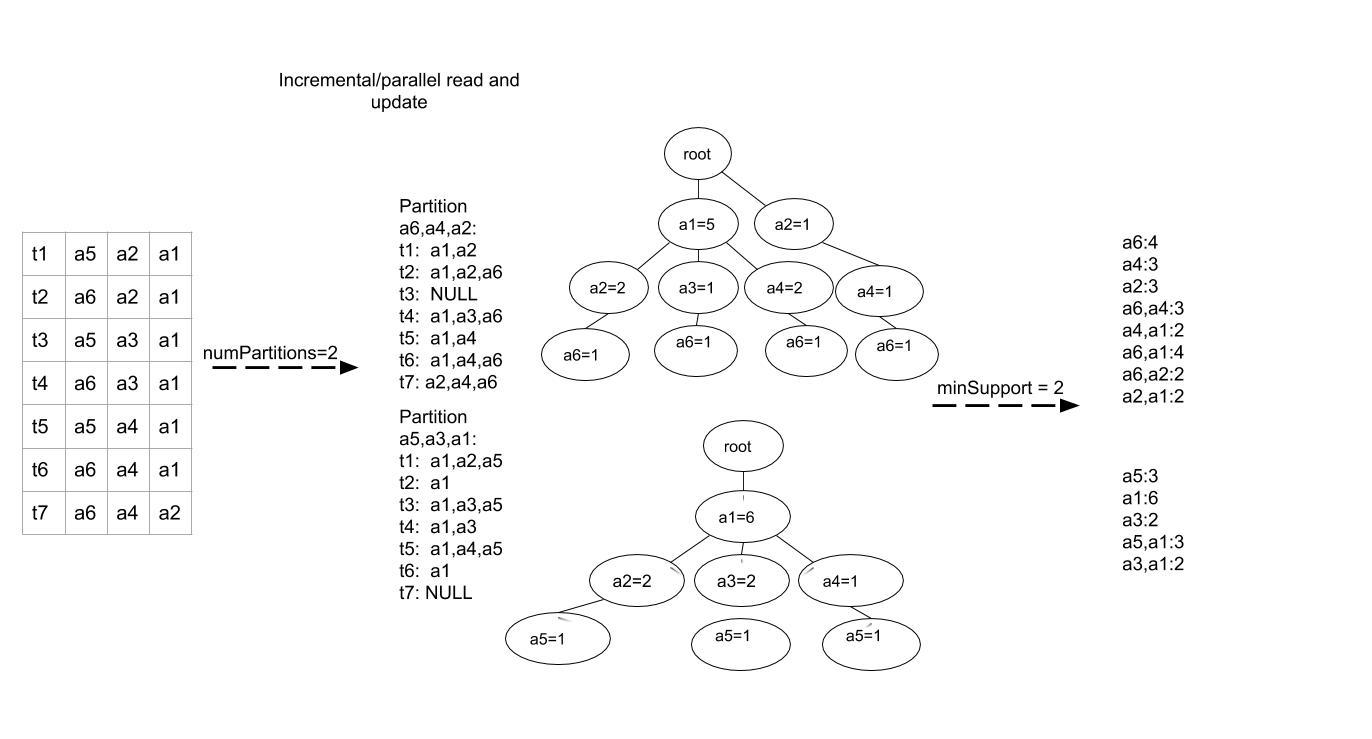
\includegraphics[width=\linewidth]{figures/IncrementalTreeMining}
  \caption{An example of trees and mining for minSup=2 and 2 partitions}
  \label{fig:incrementalParallelMining}
\end{figure}


%\begin{table*}[t]
%  \caption{A double column table.}
%  \label{tab:commands}
%  \begin{tabular}{ccl}
%    \toprule
%    A Wide Command Column & A Random Number & Comments\\
%    \midrule
%    \verb|\tabular| & 100& The content of a table \\
%    \verb|\table|  & 300 & For floating tables within a single column\\
%    \verb|\table*| & 400 & For wider floating tables that span two columns\\
%    \bottomrule
%  \end{tabular}
%\end{table*}

\subsection{Related Work}
  One of the most well known algorithms for mining association rules is the Apriori algorithm~\cite{agrawal1994fast}. This algorithm is iteratively generating candidates and pruning items with low support at each step. If an item of length N is frequent, then all sub patterns must be frequent as well. Using that idea, an early prune of non-frequent itemsets removes many unnecessary candidates in later iterations.

In the year 2000, a tree based solution was introduced, FPGrowth algorithm and structure~\cite{agrawal1994fast}. This algorithm removes the need for candidate generation and yields better performance~\cite{hunyadi2011performance}. A small example is provided in \autoref{fig:fpgrowthexample}

%Also worth mentioning the FIUT (Frequent-Item-Ultrametric-Trees) algorithm~\cite{tsay2009fiut}, which was presenter in 2009 by Y.j. Tsay, T.J. Hsu and J.R. Yu.
%This algorithm is trying to overcome one of the biggest drawbacks of the FP-Growth algorithm - the recursive calculation of the association rules. Which for large databases may not fit in a processor memory. The proposed idea to overcome this drawback, is to use trees where all paths are from the same lengths, and the leafs will be a hash of the items in the path. 
%For the incremental use case, it will require to load and update all the trees of length K till 2, where K is the size of an item in the new data arriving. This will be exhaustive and inefficient. However for the regular calculation of association rules, the FIUT performance results are significantly better than FP-Growth.

\subsection{Incremental Frequent Itemsets Mining}
The idea behind incremental calculations and updates, is to recompute outputs which depend on the incoming input only, without recomputing the whole data.

The basic challenge in incremental updates for frequent items mining, is a non consistent frequency order. Several algorithms such as AFPIM~\cite{koh2004efficient}, EFPIM~\cite{li2006fast} and FUFP-tree~\cite{hong2008incrementally} are keeping an updated frequency based trees, by reordering branches where frequency has changed.

The work of~\cite{leung2005cantree} presented a Canonical Tree (CanTree) which preserves the frequency descending structure as in FP Growth mining, by relying on a predefined order, which will not affect the tree structure and correctness.

	The work of~\cite{tanbeer2009efficient} proposes an improvement to CanTree, called CompactPattern-Tree, and discusses the memory and computation limitations of CanTree for large incremental Databases. The issues are caused due to un-efficient tree structure, and CP-Tree is proposing an improvement by periodically (using a proposed guideline) updating the order of the construction literals list (l-list) and rebuilding the trees. As mention in the original article and as seen by our experiments, the CanTree and CP-Tree has a similar tree size, and the difference for our test cases was 10\% in tree sizes. 
	
	As we will show later in the results, using an approach similar to ~\cite{kohefficient} and maintaining a pre-min support will significantly improve memory and mining results.
	

\subsection{Parallel Frequent Itemsets mining}
The difficulty in parallelizing FP-growth is to distribute iterations to parallel trees. PFP~\cite{li2008pfp} is solving this by dividing the DB transactions and the trees using a Group-List, where every group consists of items, and redistributing iterations in the DB based on this list.
PFP is working in the following steps:

\begin{steps}
	\item Find global frequency list, F-List
	\item Group items G-list
	\item PFP:
		\begin{enumerate}
			\item For each Ti, order by F-List frequency
			\item For each aj in Ti, replace aj with gi that aj belongs to its group
			\item For each gi, if it appears in Ti, find its right-most location in Ti, say L and output:
 <key'=gi; value'={Ti[0]…Ti[L]}>
 			\item Group by key' = gi
 			\item For each group gi, build appropriate tree
 			\item For each group gi, mine the generated tree (filter items not in gi).
		\end{enumerate}
\end{steps}

\begin{figure}
  \centering
  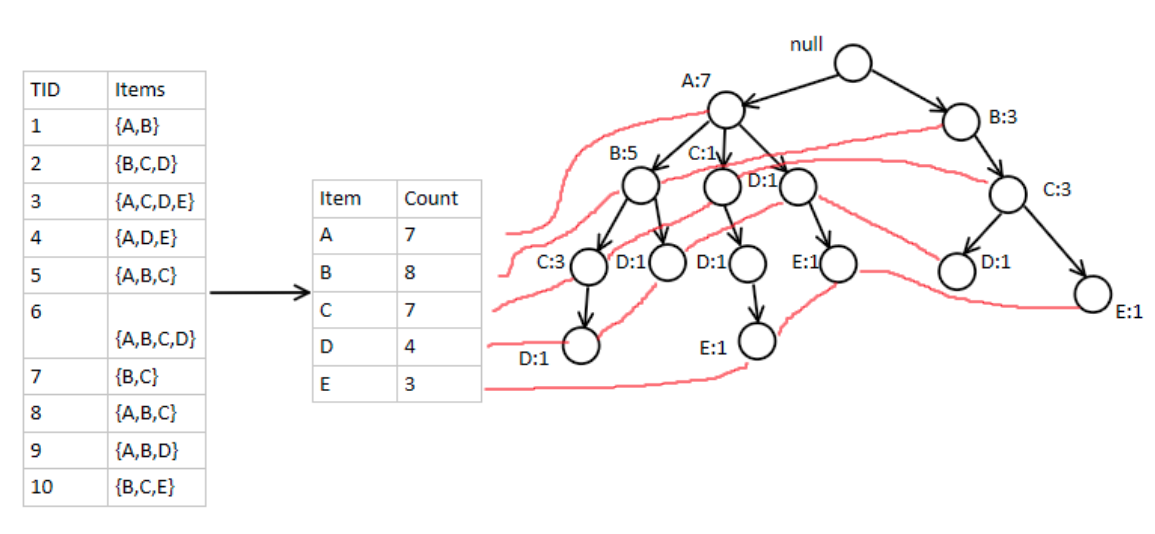
\includegraphics[width=\linewidth]{figures/fpgrowthexample}
  \caption{FPGrowth example}
  \label{fig:fpgrowthexample}
\end{figure}

It is important to mention that there might be some duplicates at several groups of frequent itemsets in stage 3.6, but this is solved when filtering the 1-length items that are not relevant to the specific group. This duplication also affects the size of the generated trees and overall memory.

\subsection{Incremental and Parallel Frequent itemsets mining}

Combining the previous 2 sections, yields an algorithm which does not rely on the frequency order and uses the parallelism advantages for computations of FIS.
The drawbacks are also drawn from the 2 algorithms - large memory consumption for saving all items and recursively calculating FIS.

\section{IPFIM - Incremental Parallel Frequent Items Mining}
The implementation of this algorithm strongly depends on PFP~\cite{li2008pfp}. To achieve support for incremental tree updates, we are using a predefined a comparison function to arrange the items, as used in CanTree~\cite{leung2005cantree}.

\subsection{IPFIM structure}
\begin{steps}
	\item Define a comparison function for items: 
	
	compare(item1,item2)->bool
	\item For each set of transactions in iteration:
		\begin{enumerate}
			\item For each Ti in current set of transaction, order by pre defined compare function.
			\item For each aj in Ti, replace aj with gi that aj belongs to its group
			\item For each gi, if it appears in Ti, find its right-most location in Ti, say L and output:
 <key'=gi; value'={Ti[0]…Ti[L]}>
 			\item Group by key' = gi
 			\item For each group gi, merge to existing tree if exists ELSE build new tree
 			\item For each group gi, mine the generated tree (filter items not in gi).
		\end{enumerate}
\end{steps}

\subsection{Correctness}
The correctness of the tree structure is driven from the correctness of mining CanTree, which preserves 2 properties:
\begin{properties}
\item \textit{The ordering of items is unaffected by the
changes in frequency caused by incremental updates.}
\item \textit{The frequency of a node in the CanTree is at
least as high as the sum of frequencies of its children.}
\end{properties}


\section{Experiments and Results}


All the test cases were divided in to 50\% base case and the remaining 50\% to iterations of 2.5\% (e.g. 20 iterations).

The implementation was done using Spark~\cite{spark}.

The used hardware is 4 clusters each with 20G memory and 40 cores. We also used SparkRDMA Plugin~\cite{SparkRDMA}.

For PFP~\cite{li2008pfp} performance comparison, Spark~\cite{spark} mllib package implements just that.

For CanTree~\cite{leung2005cantree} performance, we used IPFIM with only one group, meaning a single tree.

The comparison between CanTree~\cite{leung2005cantree} and parallel CanTree~\cite{leung2005cantree} (1, 25, 100, 1000 partitions) can be seen in \autoref{fig:IPFP1M0001}.

The comparison between IPFIM and PFP can be seen in \autoref{fig:PFPvsIPFP}.

\begin{figure}
  \centering
  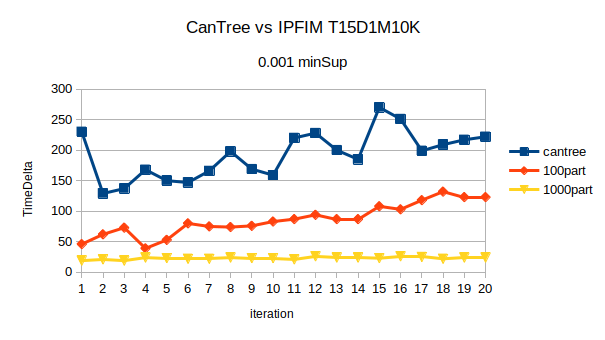
\includegraphics[width=\linewidth]{figures/IPFP1M0001}
  \caption{Inc. vs IPFIM}
  \label{fig:IPFP1M0001}
\end{figure}

\begin{figure}
  \centering
  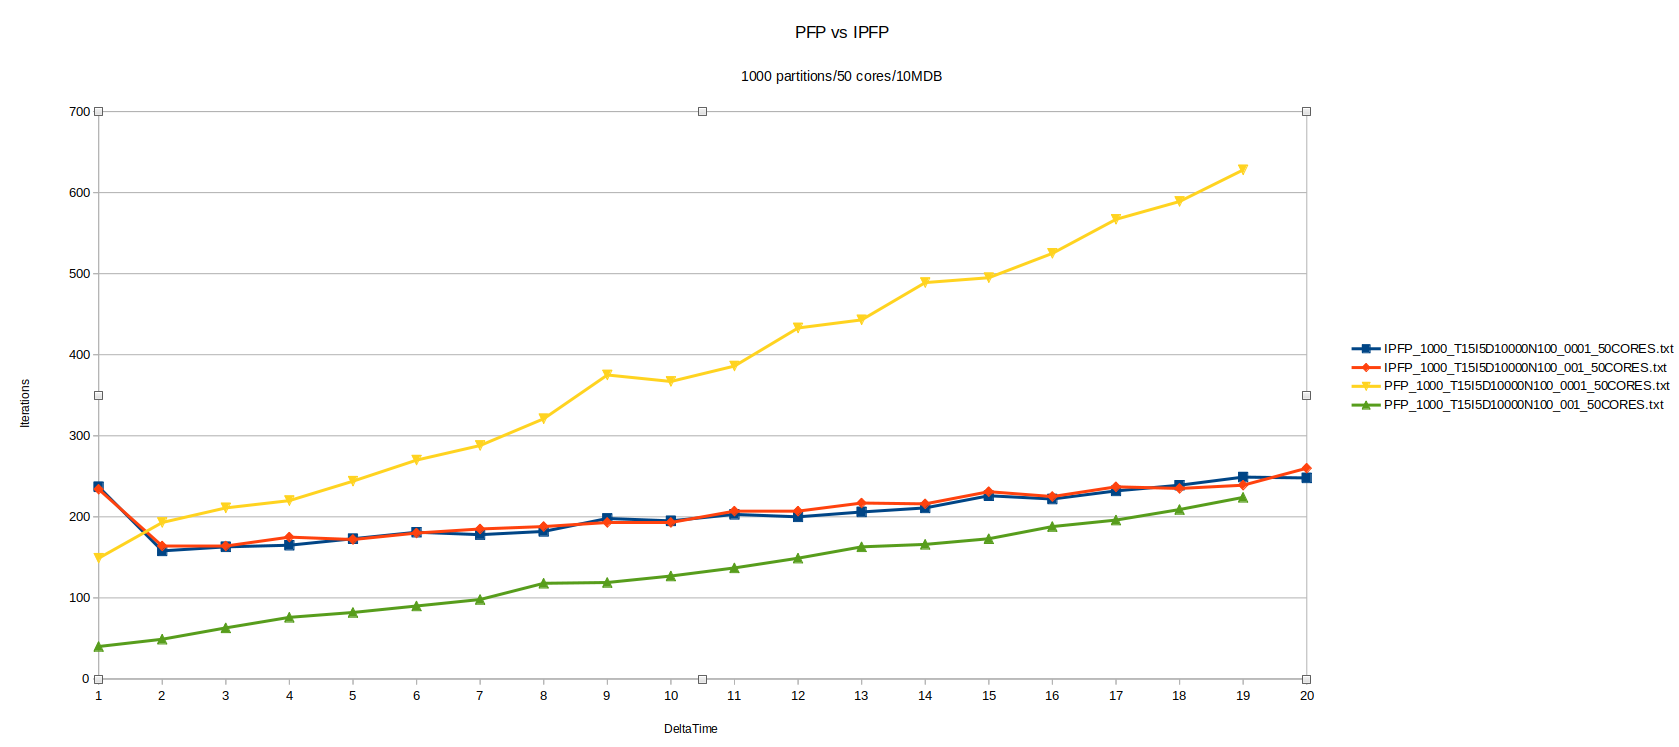
\includegraphics[width=\linewidth]{figures/PFPvsIPFP}
  \caption{PFP vs IPFIM}
  \label{fig:PFPvsIPFP}
\end{figure}


\subsubsection{IPFIM vs CanTree}
There is a XX improvement in memory (tree size) and XX in performance.
\subsubsection{IPFIM vs PFP}
When comparing large minSupport values, PFP will generate small FP-Trees and performance is significantly faster. For smaller minSupport values, the load of all dataset iterations till current point, and recalculating new FP-Tree every time, is XX times slower than IPFIM.

%\subsection{Tables}
%
%Curabitur vitae nulla dapibus, ornare dolor in, efficitur enim. Cras fermentum facilisis elit vitae egestas. Mauris porta, neque non rutrum efficitur, odio odio faucibus tortor, vitae imperdiet metus quam vitae eros. Proin porta dictum accumsan \autoref{tab:commands}.
%
%Duis cursus maximus facilisis. Integer euismod, purus et condimentum suscipit, augue turpis euismod libero, ac porttitor tellus neque eu enim. Nam vulputate est non tellus efficitur pharetra. Aenean molestie tristique venenatis. Nam congue pulvinar vehicula. Duis lacinia mollis purus, ac aliquet arcu dignissim ac \autoref{tab:freq}. 
%
%\begin{table}[hb]% h asks to places the floating element [h]ere.
%  \caption{Frequency of Special Characters}
%  \label{tab:freq}
%  \begin{tabular}{ccl}
%    \toprule
%    Non-English or Math & Frequency & Comments\\
%    \midrule
%    \O & 1 in 1000& For Swedish names\\
%    $\pi$ & 1 in 5 & Common in math\\
%    \$ & 4 in 5 & Used in business\\
%    $\Psi^2_1$ & 1 in 40\,000 & Unexplained usage\\
%  \bottomrule
%\end{tabular}
%\end{table}
%
%Nulla sit amet enim tortor. Ut non felis lectus. Aenean quis felis faucibus, efficitur magna vitae. Curabitur ut mauris vel augue tempor suscipit eget eget lacus. Sed pulvinar lobortis dictum. Aliquam dapibus a velit.
%
%\subsection{Listings and Styles}
%
%Aenean malesuada fringilla felis, vel hendrerit enim feugiat et. Proin dictum ante nec tortor bibendum viverra. Curabitur non nibh ut mauris egestas ultrices consequat non odio.
%
%\begin{itemize}
%\item Duis lacinia mollis purus, ac aliquet arcu dignissim ac. Vivamus accumsan sollicitudin dui, sed porta sem consequat.
%\item Curabitur ut mauris vel augue tempor suscipit eget eget lacus. Sed pulvinar lobortis dictum. Aliquam dapibus a velit.
%\item Curabitur vitae nulla dapibus, ornare dolor in, efficitur enim.
%\end{itemize}
%
%Ut sagittis, massa nec rhoncus dignissim, urna ipsum vestibulum odio, ac dapibus massa lorem a dui. Nulla sit amet enim tortor. Ut non felis lectus. Aenean quis felis faucibus, efficitur magna vitae. 
%
%\begin{enumerate}
%\item Duis lacinia mollis purus, ac aliquet arcu dignissim ac. Vivamus accumsan sollicitudin dui, sed porta sem consequat.
%\item Curabitur ut mauris vel augue tempor suscipit eget eget lacus. Sed pulvinar lobortis dictum. Aliquam dapibus a velit.
%\item Curabitur vitae nulla dapibus, ornare dolor in, efficitur enim.
%\end{enumerate}
%
%Cras fermentum facilisis elit vitae egestas. Mauris porta, neque non rutrum efficitur, odio odio faucibus tortor, vitae imperdiet metus quam vitae eros. Proin porta dictum accumsan. Aliquam dapibus a velit. Curabitur vitae nulla dapibus, ornare dolor in, efficitur enim. Ut maximus mi id arcu ultricies feugiat. Phasellus facilisis purus ac ipsum varius bibendum.
%
%\subsection{Math and Equations}
%
%Curabitur vitae nulla dapibus, ornare dolor in, efficitur enim. Cras fermentum facilisis elit vitae egestas. Nam vulputate est non tellus efficitur pharetra. Vestibulum ligula est, varius in suscipit vel, porttitor id massa. Cras facilisis suscipit orci, ac tincidunt erat.
%\begin{equation}
%  \lim_{n\rightarrow \infty}x=0
%\end{equation}
%
%Sed pulvinar lobortis dictum. Aliquam dapibus a velit porttitor ultrices. Ut maximus mi id arcu ultricies feugiat. Phasellus facilisis purus ac ipsum varius bibendum. Aenean a quam at massa efficitur tincidunt facilisis sit amet felis. 
%\begin{displaymath}
%  \sum_{i=0}^{\infty} x + 1
%\end{displaymath}
%
%Suspendisse molestie ultricies tincidunt. Praesent metus ex, tempus quis gravida nec, consequat id arcu. Donec maximus fermentum nulla quis maximus.
%\begin{equation}
%  \sum_{i=0}^{\infty}x_i=\int_{0}^{\pi+2} f
%\end{equation}
%
%Curabitur vitae nulla dapibus, ornare dolor in, efficitur enim. Cras fermentum facilisis elit vitae egestas. Nam vulputate est non tellus efficitur pharetra. Vestibulum ligula est, varius in suscipit vel, porttitor id massa. Cras facilisis suscipit orci, ac tincidunt erat.

\section{Conclusions}
From the results, there is a memory limitation when building trees with full items to support interactive transactions. Splitting to multiple partitions and calculations will improve memory and runtime performance, but is also limited by the number of processors.


\begin{acks}
 This work was supported by the [...] Research Fund of [...] (Number [...]). Additional funding was provided by [...] and [...]. We also thank [...] for contributing [...].
\end{acks}

%\clearpage

\bibliographystyle{ACM-Reference-Format}
\bibliography{sample}

\end{document}
\endinput
